\subchapter{Init script optimizations}{Analysing and optimizing init
scripts}

\section{Measuring}

Remember that the first step in optimization work is measuring elapsed
time. We need to know which parts of the init scripts are the biggest
time consumers.

\subsection{Use bootchartd on the board}

Add \code{bootchartd} to your \code{BusyBox} configuration
\footnote{Hint: to find where \code{bootchartd} support can be
added in the \code{BusyBox} configuration interface, press the \code{/}
key (search command). This will tell you in which submenu the
corresponding option can be found.}.

\begin{verbatim}
cd /opt/boot-time-labs/buildroot/buildroot-at91/
make busybox-menuconfig
make
\end{verbatim}

The above command should only take a few seconds to run.

\subsection{Re-flash the root filesystem}

Reflash your root filesystem in the same way you did it in the previous
labs. Reboot it as usual to let it generate its SSH keys.

The next thing to do is to use the \code{init} argument on the
kernel command line (in \code{u-boot}, this is the \code{bootargs}
environment variable) to boot using \code{bootchart} instead of using
the \code{init} program provided by Busybox.

To go to the \code{u-boot} prompt, go to the \code{picocom} window
showing the boards's serial line, reset your board with \code{PB1}, and
press a key before the timer expires.

First, have a look at the current value of the \code{bootargs}
environment variable:

\begin{verbatim}
U-Boot> printenv bootargs
bootargs=console=ttyS0,115200
mtdparts=atmel_nand:8M(bootstrap/uboot/kernel)ro,-(rootfs) rw
rootfstype=ubifs ubi.mtd=1 root=ubi0:rootfs
\end{verbatim}

Now add the \code{init} kernel parameter as follows:

\begin{verbatim}
U-Boot> setenv bootargs ${bootargs} init=/sbin/bootchartd
U-Boot> saveenv
U-Boot> boot
\end{verbatim}

This will make the system boot and the resulting bootlog will be located
in \code{/var/log/bootlog.tgz}. Copy that file on your host. You can do
this by inserting the USB disk provided by your instructor into one of
the USB hosts ports of the board:

\begin{verbatim}
# mount /dev/sda1 /mnt
# cp /var/log/bootlog.tgz /mnt
# umount /mnt
\end{verbatim}

\section{Analyse bootchart data on your workstation}

To use \code{bootchart} on your workstation, you first need to
install a few Java packages:

\begin{verbatim}
sudo apt-get install ant openjdk-6-jdk
\end{verbatim}

Now, get the \code{bootchart} source code
\footnote{The source code was originally found on
\url{http://prdownloads.sourceforge.net/bootchart/bootchart-0.9.tar.bz2}.}
\footnote{Don't try to get the \code{bootchart} package supplied by
Ubuntu instead. While it has similar functionality, it looks like a completely
unrelated piece of software. To confirm this, it has no dependency
whatsoever on Java packages.}
, compile it and use \code{bootchart} to generate the boot
chart:

\begin{verbatim}
cd /opt/boot-time-labs/buildroot/
cp /media/BootTime/downloads/bootchart-0.9.tar.bz2 .
tar xf bootchart-0.9.tar.bz2
cd bootchart-0.9
ant
java -jar bootchart.jar /media/BootTime/bootlog.tgz
\end{verbatim}

This produces the \code{bootlog.png} image which you can visualize to
study and optimize your startup sequence:

\begin{verbatim}
xdg-open bootlog.png
\end{verbatim}

\code{xdg-open} is a universal way of opening a file with a given MIME
type with the associated application as registered in the system.
According to the exact Ubuntu flavor that you are using (Ubuntu,
Xubuntu, Kubuntu...), it will run the particular image viewer available in that
particular flavor.

\begin{center}
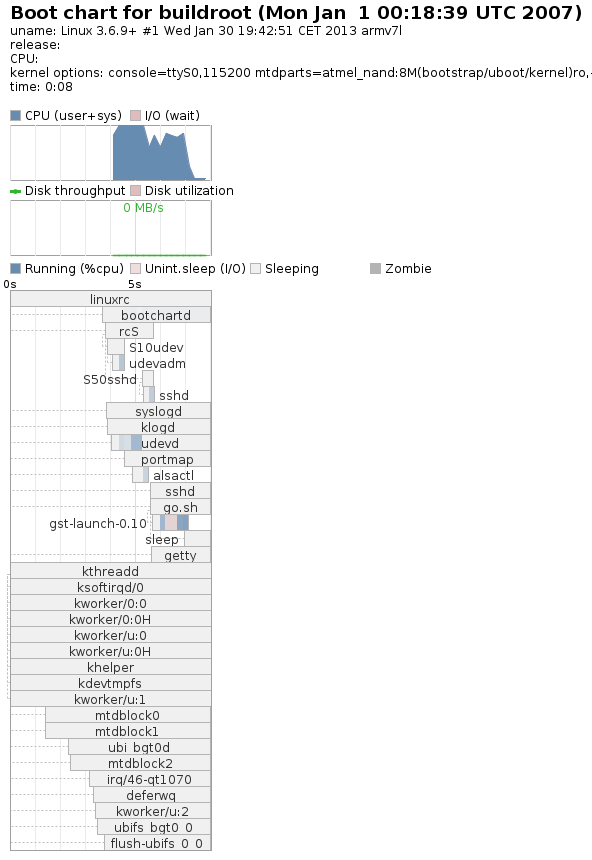
\includegraphics[width=8cm]{labs/boottime-init-scripts/bootlog.png}
\end{center}

\section{Remove unnecessary functionality}

The above graph shows that there are \code{udev} processes running
during the startup process, taking a significant amount of CPU time
(the graph shows blue rectanges when the processes actually uses
the CPU).

\code{udev} is pretty likely to be unnecessary in this system. Managing
device files (even for hotplugged devices) is perfectly taken care
of by the kernel's \code{devtmpfs} filesystem. \code{udev} might be
needed to run specific programs to react to hotplugging events, but
it has no visible usefulness in the basic demo usage scenario.

So let's remove \code{udev}! To do so, disable it in the Buildroot
configuration:

\begin{verbatim}
cd /opt/boot-time-labs/buildroot/buildroot-at91/
make menuconfig
\end{verbatim}

In \code{System configuration} and then in \code{/dev management},
choose \code{Dynamic using devtmpfs only}.

The next step would be to re-run Buildroot. However, we're hitting one
of the current limitations of Buildroot. To keep its design simple and
efficient, Buildroot currently doesn't support removing software
even if it has been removed from the configuration. The clean way
{\em would} be to run \code{make clean} and then run \code{make}
again.

This is usually fine, as Buildroot is pretty fast. In our case however,
we made it Buildroot build its own toolchain, and doing this is the most
time consuming part. We would lose a lot of time.

So, let's remove \code{udev} manually instead. Again, this is a quick
and dirty trick to save time in a time limited workshop. Don't do this
for a production project! It may have unexpected side effects.

\begin{verbatim}
find output/target/ -name "*udev*"
rm -r output/target/etc/udev/
rm output/target/etc/init.d/S10udev
rm output/target/usr/lib/libudev.so
rm output/target/usr/bin/udevadm
rm -r output/target/lib/udev/
rm output/target/lib/libudev.so.0*
\end{verbatim}

Let's also take this opportunity to disable \code{bootchartd}
compilation. Do this through \code{make busybox-menuconfig}, and remove
the \code{output/target/sbin/bootchartd} file manually.

Rebuild your root filesystem (run \code{make}) and reflash the device once again.
You don't have to worry about removing \code{bootchartd} from the kernel
command line as the flashing process got you back to the initial kernel
command line.

After the first reboot (as always for SSH key generation), reboot your
board through \code{grabserial} and measure the time stamp for the
\code{Done playing video} message.

\section{Postpone services}

If we get back to the bootchart that we generated, we can see that there
are several other services which might be needed for the device to
have all its features, but which should be run after the demo video,
instead of before it. One example is the SSH server.

Let's customize the \code{/etc/init.d/rcS} file which starts such
services, in order to start the video player first, and the other services
later.

First, let's make a copy of what Buildroot generated:

\begin{verbatim}
cp output/target/etc/init.d/rcS board/atmel/sama5d3ek_demo/
\end{verbatim}

Then, add the below lines after the first line in this copy:

\begin{verbatim}
/root/go.sh &
sleep 5
\end{verbatim}

The first added line corresponds to the contents of
\code{/etc/init.d/S99demo}. We remove this executable, because
we will continue to use the \code{S??*} wildcard to start the
other services.

According to the measures we have already made, the delay of 5 seconds
should be more than enough to let the player play the 1 frame video.
With this pessimistic delay, we make sure that the CPU will only be
dedicated to the video player for 3 seconds.

Now, let's copy this replacement \code{/etc/init.d/rcS} file by
modifying \code{board/atmel/sama5d3ek_demo/post-build.sh} once again:

\begin{itemize}
\item By removing the code that creates \code{/etc/init.d/S99demo}
\item By coping our new \code{rcS} file to the target filesystem.
\end{itemize}

The last thing to do before running \code{make} is to remove the
\code{output/target/etc/init.d/S99demo} file manually. Remember that
Buildroot doesn't clean the target directory!

Now run \code{make} and make sure that
\code{output/target/etc/init.d/rcS} has the new right contents.

Reflash your system, and reboot it through \code{grabserial} to
measure the new total boot time.
\footnote{Note that we are no longer bothered by SSH key generation,
as it starts after our video is played. Therefore, one reboot
after reflashing is now sufficient.}

Write down your results in the table at the end of this chapter.

While the total boot time is now smaller, you can still notice
that the time to run the player is slightly longer. It's not surprising.
You can guess that the video player is sharing some libraries (mainly C
library components) with the executables for the other services. Since
the services are no longer started before itself, it must be the first
one to load such libraries, which explains the longer time to start.

\section{Optimize necessary functionality}

It's now time to optimize the \code{go.sh} script that runs the video,
by making this script as simple as possible.

\subsection{Simplify shell programming}

First, let's make a simple, one-time experiment that we won't keep.
Directly on the board, modify \code{/root/go.sh}, replacing

\begin{verbatim}
while `ls /dev/fb0 > /dev/null 2>&1`
\end{verbatim}

by

\begin{verbatim}
while [ -e /dev/fb0 ]
\end{verbatim}

This is a much simpler test, with no output to manage. It is even
very likely that the test command is a shell built-in, meaning that
there is no sub-process to spawn (very costly).

Run \code{halt} and then reboot the board with \code{grabserial},
and measure how much time you saved by simplifying this test.
In our own tests, we saved 34 ms! This is not negligible at all
when similar cases accumulate and you are aiming at booting in just
a few seconds.

The lesson to learn is that the shell scripts should be programmed
with very good care, to avoid complex constructs causing multiple
children processes to be run while fewer would be sufficient.

\subsection{Radical simplification of the launcher script}

Now, let's make \code{/root/go.sh} as simple as possible:

\begin{itemize}
\item By removing the soc subtype check.
      This check was very complex, and completely unnecessary
      when you have the video capable SoC.
\item By running the video player just once, instead of through
      an endless \code{while} loop.
\end{itemize}

Simplify the contents of this file by removing lines
in \code{board/atmel/sama5d3ek_demo/post-build.sh}.

As usual, update your root filesystem, reflash it, measure the
new results and store them in the table below.

\subsection{Going further}

If you are ahead of the others in the workshop, there are
other thing you could try to do to start the video player earlier: You could

\begin{itemize}
\item Take the commands that are run before \code{/etc/init.d/rcS} in
      \code{/etc/inittab}, and move them after starting the video in
      \code{/etc/init.d/rcS}.
\item In \code{/etc/init.d/rcS}, source \code{/root/go.sh} instead of
      executing it. This way, this shell script will be interpreted
      by the current shell, instead of having to spawn a child process
      (another shell, this is expensive).
\end{itemize}

Last but not least, there's another thing we can simplify. We could
recompile \code{BusyBox} with only the capabilities that are needed
in this demo. It would make the \code{init} program and the other
executables faster to load (being smaller) and run.

However, we prefer to make such a simplification at the end, because
it is convenient to interact with a full-featured set of UNIX commands
when you experiment with your system.

\section{Results}

Fill the below table with the results from your experiments:

\begin{tabular}{| l | c | c | r |}
  \hline
  Technique & Total time stamp & Difference with previous
experiment \\
  \hline
  \hline
  Original time & & N/A \\
  \hline
  Remove \code{udev} & & \\
  \hline
  Postpone services & & \\
  \hline
  Optimize launcher & & \\
  \hline
  Other trick & & \\
  \hline
  Other trick & & \\
  \hline
  \hline
  \multicolumn{2}{| c |}{Total gain} & \\
  \hline
\end{tabular}


